\subsection{Криволинейные координаты}

\subsubsection*{Т1.}

Найдём коварианные и контрвариантные компоненты $\vc{a}$. Учитывая, что тензор однозначно задаётся координатами в некотором базисе:
$$
    \letus \vc{b} = a^i \vc{g}_i \hspace{0.25cm} \big|_{\cdot \vc{g}^j}
    \hspace{0.5cm} \Rightarrow \hspace{0.5cm}  
    (\vc{b} \cdot \vc{g}^j) = a^i (\vc{g}_i \cdot \vc{g}^j) = a^i \delta_i^j = a^j
    \hspace{0.5cm} \Rightarrow \hspace{0.5cm} a^i \vc{g}_i = \vc{a}.
$$
Аналогично
$$
    \letus \vc{b} = a_i \vc{g}^i \hspace{0.25cm} \big|_{\cdot \vc{g}_j}
    \hspace{0.5cm} \Rightarrow \hspace{0.5cm} 
    (\vc{b} \cdot \vc{g}_j) = a_i (\vc{g}^i \cdot \vc{g}_j) = a_i \delta_j^i = a_j
    \hspace{0.5cm} \Rightarrow \hspace{0.5cm} a_i \vc{g}^i = \vc{a}.
$$
Теперь научимся жонглировать индексами. 
$$
    \letus \vc{b}^i = g^{ij} \vc{g}_j \hspace{0.25cm} \big|_{\cdot \vc{g}^n} \hspace{0.5cm} \Rightarrow \hspace{0.25cm} 
    g^{ij} \vc{g}_g \vc{g}^n = g^{ij} \delta^n_j = g^{in} =  (\vc{k}^i \cdot \vc{g}^n)
    \hspace{0.5cm} 
    \Rightarrow
    \hspace{0.5cm} 
    \vc{g}^i = g^{ij} \vc{g}_j.
$$
Для $g_{ij} \vc{g}^{j} = \vc{g}_i$ доказательство аналогично. Наконец,
$$
    \delta_i^j = (\vc{g}_i \cdot \vc{g}^j) = \left(
        g_{ik} \vc{g}^k \cdot g^{jn} \vc{g}_n
    \right) = g_{ik} g^{jn} \delta_n^k = g_{ik} g^{kj}.
$$
Теперь, для жонглирования над координатой:
$$
    \letus \vc{a} = a_i \vc{g}^i \hspace{0.25cm} \big|_{\cdot \vc{g}^j}
    \hspace{0.5cm} \Rightarrow \hspace{0.5cm}   
    a^j = g^{ij} a_i.
$$

\subsubsection*{Т2.}
Найдём локальный базис/матрицу перехода из ПДСК для $\vc{r}(\sigma, \tau, z)$:
$$
    \vc{r}(\sigma, \tau, z) =
    \begin{pmatrix}
        \sigma\tau \\ (\tau^2 - \sigma^2)/2 \\ z
    \end{pmatrix};
    \hspace{0.5cm} 
    \vc{g}_i = \frac{\partial \vc{r}}{\partial q^i} 
    \hspace{0.25cm} \Rightarrow \hspace{0.25cm} 
    \vc{J} = 
    \begin{pmatrix}
        \tau & \sigma & 0 \\
        -\sigma & \tau & 0 \\
        0 & 0 & 1
    \end{pmatrix};
    \hspace{0.25cm} 
    g_{ij} = \vc{J}\T \vc{J} = \diag (\tau^2 + \sigma^2, \tau^2 + \sigma^2, 1).
$$
Зафиксировав значения всех кроме одной переменных найдём координатные линии, затем построим координатные поверхности (см. рис. \ref{fig:1}).
\begin{figure}[h]
    \centering
    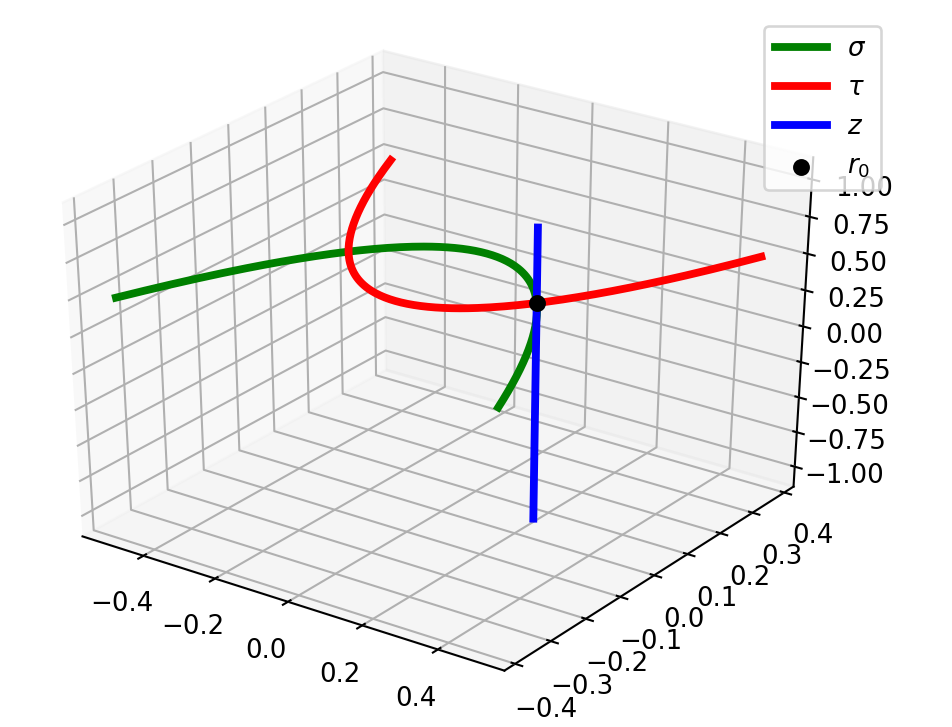
\includegraphics[width=0.4\textwidth]{img/1_2.png}
    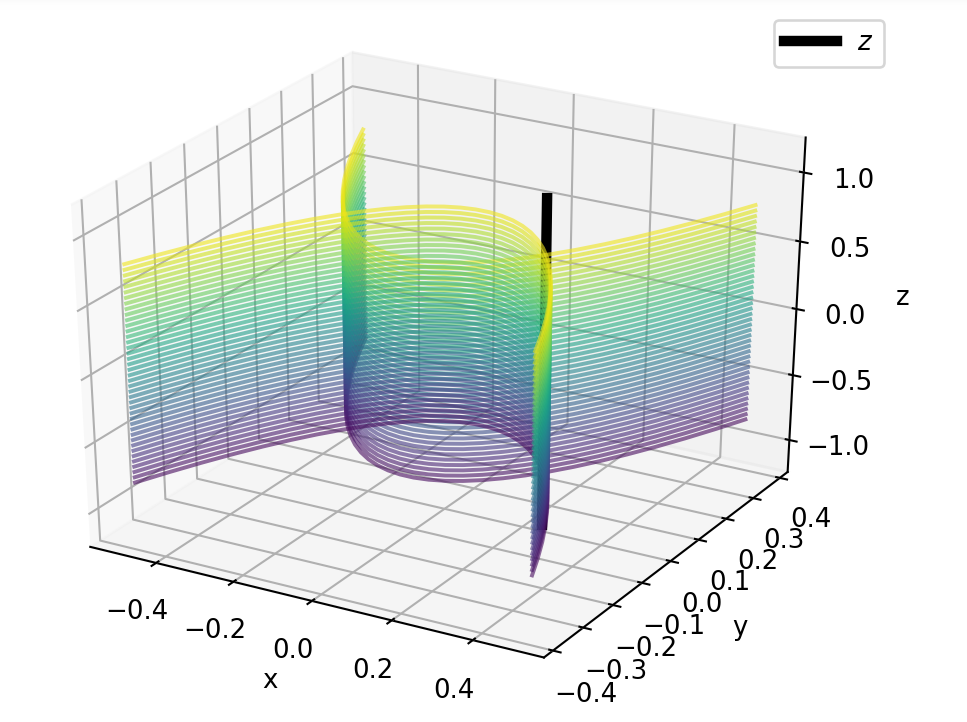
\includegraphics[width=0.4\textwidth]{img/1_2_2.png}
    \caption{Координатные линии и координатные поверхности.}
    \label{fig:1}
\end{figure}

\subsubsection*{Т3.}

Найдём метрический тензор $g_{ij}$ для криволинейных координат 
$(r, \varphi)$, задающих положение точки на параболоиде $z = a(x^2 - y^2)$, при $a=\const$, $x = r \cos \varphi$, $y = r \sin \varphi$.
$$
    \vc{r} = \begin{pmatrix}r \cos{\left(\varphi \right)}\\r \sin{\left(\varphi \right)}\\a r^{2} \cos{\left(2 \varphi \right)}\end{pmatrix};
    \hspace{0.5cm} 
    \vc{g}_i = \frac{\partial \vc{r}}{\partial q^i} 
    \hspace{0.25cm} \Rightarrow \hspace{0.25cm} 
    g_r =\begin{pmatrix}\cos{\left(\varphi \right)}\\\sin{\left(\varphi \right)}\\2 a r \cos{\left(2 \varphi \right)}\end{pmatrix};
    \hspace{0.25cm} 
    g_{\varphi} = \begin{pmatrix}- r \sin{\left(\varphi \right)}\\r \cos{\left(\varphi \right)}\\- 2 a r^{2} \sin{\left(2 \varphi \right)}\end{pmatrix}
$$
Тогда метрический тензор:
\begin{align*}
        g_{ig} &= (\vc{g}_i \cdot \vc{g}_j); \\ 
        g_{11} &= 4 a^{2} r^{2} \cos^{2}{\left(2 \varphi \right)} + \sin^{2}{\left(\varphi \right)} + \cos^{2}{\left(\varphi \right)}; \\
        g_{12} &= g_{21} = - 2 a^{2} r^{3} \sin{\left(4 \varphi \right)}; \\
        g_{22} &= 4 a^{2} r^{4} \sin^{2}{\left(2 \varphi \right)} + r^{2} \sin^{2}{\left(\varphi \right)} + r^{2} \cos^{2}{\left(\varphi \right)}.
\end{align*}
Объединяя, 
$$
    g_{ij} = \begin{pmatrix}16 a^{2} r^{2} \sin^{4}{\left(\varphi \right)} - 16 a^{2} r^{2} \sin^{2}{\left(\varphi \right)} + 4 a^{2} r^{2} + 1 & - 2 a^{2} r^{3} \sin{\left(4 \varphi \right)}\\- 2 a^{2} r^{3} \sin{\left(4 \varphi \right)} & - 16 a^{2} r^{4} \sin^{4}{\left(\varphi \right)} + 16 a^{2} r^{4} \sin^{2}{\left(\varphi \right)} + r^{2}\end{pmatrix}.
$$
Или,
$$
    g^{ij} = (g_{ij})^{-1} = \begin{pmatrix}\frac{- 16 a^{2} r^{2} \sin^{4}{\left(\varphi \right)} + 16 a^{2} r^{2} \sin^{2}{\left(\varphi \right)} + 1}{4 a^{2} r^{2} + 1} & \frac{2 a^{2} r \sin{\left(4 \varphi \right)}}{4 a^{2} r^{2} + 1}\\\frac{2 a^{2} r \sin{\left(4 \varphi \right)}}{4 a^{2} r^{2} + 1} & \frac{16 a^{2} r^{2} \sin^{4}{\left(\varphi \right)} - 16 a^{2} r^{2} \sin^{2}{\left(\varphi \right)} + 4 a^{2} r^{2} + 1}{4 a^{2} r^{4} + r^{2}}\end{pmatrix}.
$$
Соответсвенно,
$$
    \vc{g}^r = g^{rr} g_{r} + g^{r\varphi} g_{\varphi} = 
    \begin{pmatrix}\frac{\left(8 a^{2} r^{2} \sin^{2}{\left(\varphi \right)} + 1\right) \cos{\left(\varphi \right)}}{4 a^{2} r^{2} + 1}\\\frac{\left(8 a^{2} r^{2} \cos^{2}{\left(\varphi \right)} + 1\right) \sin{\left(\varphi \right)}}{4 a^{2} r^{2} + 1}\\\frac{2 a r \cos{\left(2 \varphi \right)}}{4 a^{2} r^{2} + 1}\end{pmatrix};
    \hspace{0.5cm} 
    \vc{g}^{\varphi} = = g^{\varphi r} g_{r} + g^{\varphi \varphi} g_{\varphi} =
    \begin{pmatrix}\frac{\left(- 8 a^{2} r^{2} \sin^{2}{\left(\varphi \right)} + 4 a^{2} r^{2} - 1\right) \sin{\left(\varphi \right)}}{r \left(4 a^{2} r^{2} + 1\right)}\\\frac{\left(8 a^{2} r^{2} \cos^{2}{\left(\varphi \right)} - 4 a^{2} r^{2} + 1\right) \cos{\left(\varphi \right)}}{r \left(4 a^{2} r^{2} + 1\right)}\\- \frac{2 a \sin{\left(2 \varphi \right)}}{4 a^{2} r^{2} + 1}\end{pmatrix}.
$$
На всякий случай проверим в \textit{SymPy}, что
$$
    \vc{g}_r \vc{g}^r = 1; \hspace{0.5cm} 
    \vc{g}_\varphi \vc{g}^{\varphi} = 1; \hspace{0.5cm} 
    \vc{g}_r \vc{g}^{\varphi} = 0; \hspace{0.5cm} 
    g^{ij} g_{ji} = \delta_i^j.
$$
Вот.

\subsubsection*{Т4.} % см. частные производные, когда что-то от чего-то зависит.

Пусть $R = x^2 + y^2 + z^2$, найдём частную производную $\partial R / \partial x$тогда
\begin{enumerate}
    \item $R(x, y, z) = x^2 + y^2 + z^2$. \hfill
        $\partial R / \partial x = 2x$.
    \item $R(x, r, z) = r^2 + z^2$. \hfill
        $\partial R / \partial x = 0$. 
    \item $R(x, y) = x^2 + y^2 + (x^2 - y^2)^2$. \hfill
        $\partial R / \partial x = 2x + 4x(x^2-y^2)$.
    \item $R(x, r) = r^2 + (x^2 - y^2)^2 = r^2 + (2x^2 - r^2)^2$. \hfill
        $\partial R / \partial x = 16x^3 - 8xr^2$.
    \item $R(x, z) = x^2 + (x^2-z) + z^2 = 2x^2 - z + z^2$.\hfill
        $\partial R / \partial x = 4x$.
\end{enumerate}


\subsubsection*{Т5.}
Для первого выражения, обозначим $(\vc{g}_i \cdot \frac{\partial \vc{g}^j}{\partial q^k}) \overset{\mathrm{def}}{=} \Xi_{ik}^j$. 
$$
    \Gamma_{ijk} = \left(\vc{g}_i, \frac{\partial \vc{g}_j}{\partial q^k}\right) 
    = \left(\vc{g}_i, \frac{\partial (g_{jn}\vc{g}^n)}{\partial q^k}\right) =
    g_{jn}\underbrace{\left(\vc{g}_i \cdot \frac{\partial \vc{g}^n}{\partial q^k} \right)}_{\Xi_{ik}^j} +
    \frac{\partial g_{jn}}{\partial q^k} \underbrace{\left(\vc{g}_i \cdot \vc{g}^n\right)}_{\delta_i^n} = g_{jn} \Xi_{ik}^j + \underbrace{\Gamma_{ijk} + \Gamma_{jik}}_{\partial g_{jn} / \partial q^k}.
$$
Домножив обе части на $g^{nj}$, получим
$$
    \Xi_{ik}^j g_{jn} g^{nj} = \boxed{(\vc{g}_i \cdot \frac{\partial \vc{g}^j}{\partial q^k}) = - \Gamma_{jik} g^{jn}}
$$


% \begin{equation}
%     \left.\begin{aligned}
%         \frac{\partial \vc{g}^j}{\partial q^k} = \frac{\partial g^{ij}}{\partial q^k} \vc{g}_i + \frac{\partial \vc{g}_i}{\partial q^k} g^{ij}; \\ 
%         \vc{g}_i \frac{\partial (\vc{g}^j \cdot \vc{g}^i)}{\partial q^k} = 
%         \delta_i^i \frac{\partial \vc{g}^j}{\partial q^k} + \frac{\partial \vc{g}^i}{\partial q^k} \delta_i^j
%         = 
%         2 \frac{\partial \vc{g}^j}{\partial q^k}
%     \end{aligned}\right\}
%     \hspace{0.25cm} \Rightarrow \hspace{0.25cm} 
%     2 \left(\vc{g}_i \cdot \frac{\partial \vc{g}^j}{\partial q^k} \right) + \Gamma_{ijk} g^{ij} = \left(\vc{g}_i  \cdot \frac{\partial \vc{g}^j}{\partial q^k} \right)
%     \hspace{0.25cm} \Rightarrow \hspace{0.25cm} 
%     (1) = - \Gamma_{ijk} g^{ij}.
% \end{equation}

Для второго выражения рассмотрим значение квадрата произведения при фиксированных $i \neq j \neq k$:
$$
    \underbrace{(\vc{g}_i, \vc{g}_j, \vc{g}_k)^2}_{\det g_{mn}} \cdot 
    \underbrace{(\vc{g}^i, \vc{g}^j, \vc{g}^k)^2}_{\det g^{nk}} = \det g_{mn} g^{np} = \det \delta_m^p = 1.
    \hspace{0.5cm} \Rightarrow \hspace{0.5cm} 
    (\vc{g}_i, \vc{g}_j, \vc{g}_k) \cdot (\vc{g}^i, \vc{g}^j, \vc{g}^k) = 3! = 6.
$$
Важно заметить, что $-1$ не является возможным значением произведения таких смешанных произведений, т.к. левой тройке в первом сомножители будет соответствовать тройка во втором сомножителе.
